\section{Closing Remarks}
\frame{\tableofcontents[currentsection]}

\begin{frame}{Acknowledgements}
\begin{figure}
    \centering
    \begin{subfigure}[b]{0.3\textwidth}
        \centering
        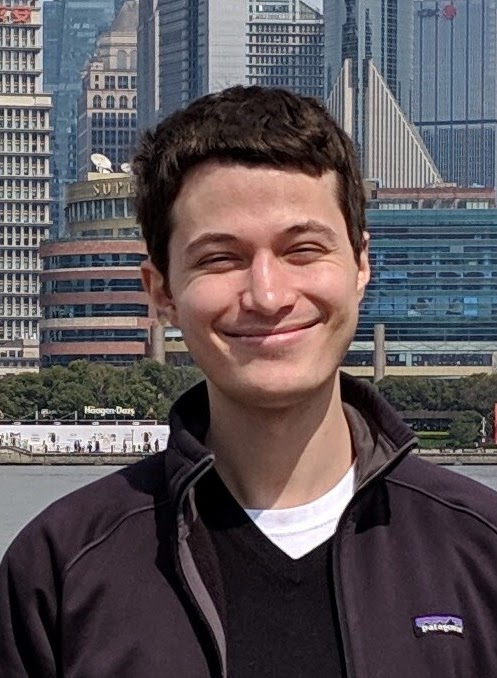
\includegraphics[width=\textwidth]{figures/alex-constantino.jpeg}
        \caption{Alex Constantino}
    \end{subfigure}
    \hfill
    \begin{subfigure}[b]{0.3\textwidth}
        \centering
        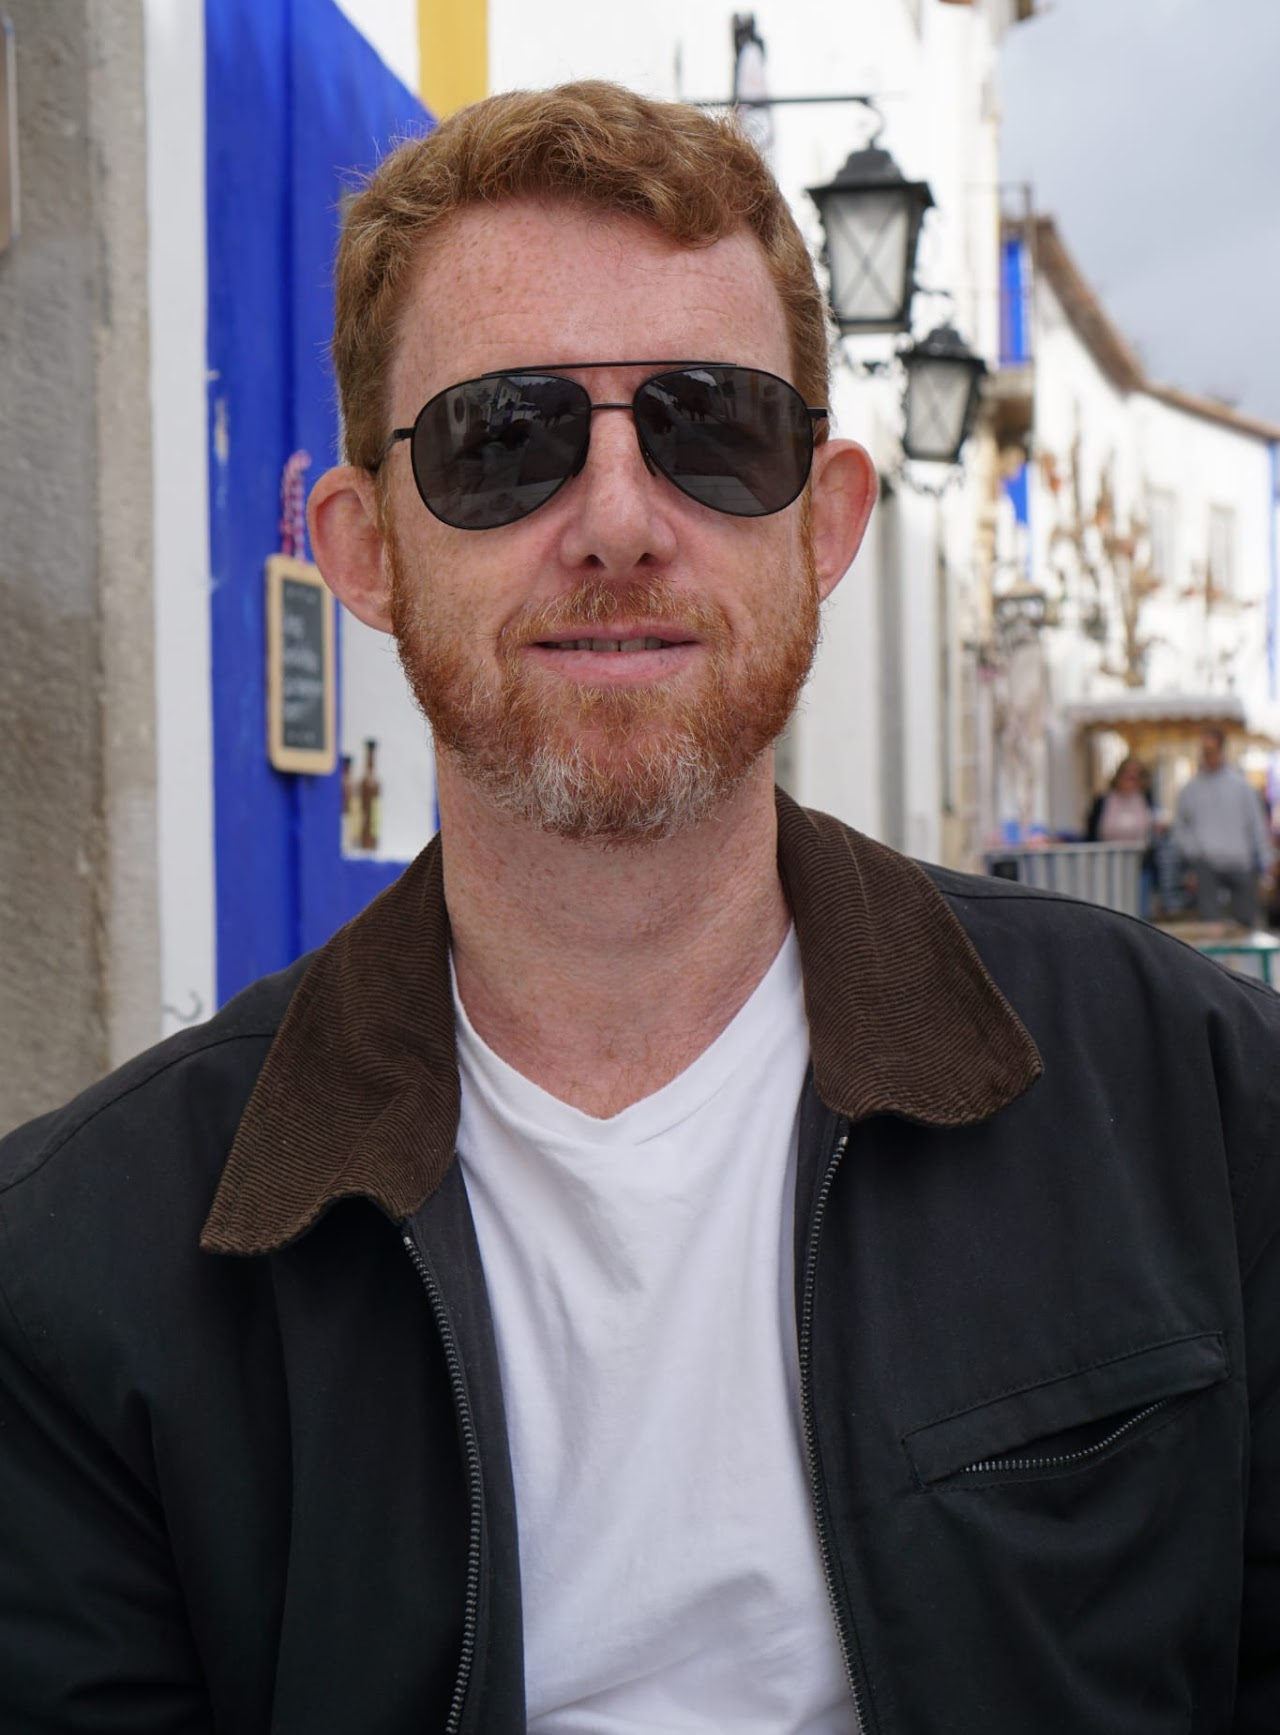
\includegraphics[width=\textwidth]{figures/gary-mulder.jpeg}
        \caption{Gary Mulder}
    \end{subfigure}
    \hfill
    \begin{subfigure}[b]{0.3\textwidth}
        \centering
        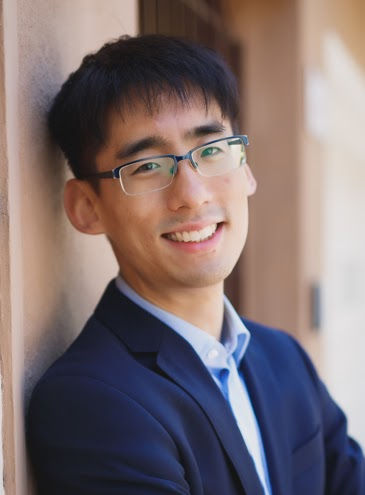
\includegraphics[width=\textwidth]{figures/daniel-kang.jpeg}
        \caption{Daniel Kang}
    \end{subfigure}
\end{figure}
\end{frame}

\begin{frame}{Recap}
\begin{itemize}
    \item Our methodology gives provable control of Type I Error via simulation.
    \item Allows complex designs to be studied seamlessly.
    \item Our software can make simulations extremely fast.
\end{itemize}
\end{frame}
